% !TEX root = main.tex

%%%%%%%%%%%%%%%%%%%%%%%%%%%%%%%%%%%%%%%%%%%%%%%%%%%%%%%%%%%%%%%%%%%%%%%%%%%%%%%%%%%%%%%%%%%%%%%%
\section{データ解析と考察}
%%%%%%%%%%%%%%%%%%%%%%%%%%%%%%%%%%%%%%%%%%%%%%%%%%%%%%%%%%%%%%%%%%%%%%%%%%%%%%%%%%%%%%%%%%%%%%%%
\begin{enumerate}
    \item 実験課題1で得られた結果から,ソレノイド中心軸上の軸方向磁束密度分布
    $B_z(z)$を算出せよ.ただし,導出過程も示すこと.
    \begin{description}
        \item[] 各$z$座標における磁気プローブの出力$V_{co}$を積分し,
        $\int_{0}^{t} V_{co}(t)dt$を算出する.その後,ソレノイド中心軸上の軸方向磁束密度分
        布$B_z(z)$を以下の式で求め,算出結果を有効数字3桁で表3に示す。
        $$
        B=-\frac{1}{NS}\int_{0}^{t} V_{co}(t)dt
        $$
        ただし、各パラメータは次のようになる.
        $$
        N=33\,[回],S=\pi \times 0.00275^2 \simeq 2.38\times 10^{-5}\,[\si{m^2}]
        $$
        \begin{table}[H]
            \centering
            \caption{ソレノイド中心軸上の軸方向磁束密度分布$B_z(z)$}
            \begin{tabular}{c|c}
            \hline
            $z座標\,[\si{cm}]$ & 磁束密度$B_z(z)\,[\si{mT}]$ \\ \hline
                -8 & 0.0900 \\ 
                -6 & 0.196 \\ 
                -4 & 0.282 \\
                -2 & 0.537 \\ 
                0 & 1.01 \\ 
                2 & 1.46 \\ 
                4 & 1.79 \\ 
                6 & 1.86 \\ 
                8 & 1.87 \\ 
                10 & 1.91 \\ 
                12 & 1.93 \\ 
                14 & 1.93 \\
                16 & 1.90 \\ 
                18 & 1.87 \\ 
                20 & 1.77 \\ 
                22 & 1.32 \\ 
                24 & 0.980 \\ 
                26 & 0.503 \\ 
                28 & 0.429 \\ 
                30 & 0.652 \\ 
                32 & 0.754 \\ \hline
            \end{tabular}
        \end{table}
    \end{description}

    \newpage

    \item ソレノイド中心軸上の軸方向磁束密度分布$B_z(z)$をビオ・サバールの法則
    を用いて計算せよ.ただし,ビオ・サバールの法則を明確に示し,そこからソレノイド
    中心軸上の磁束密度を求める導出過程も詳細に記述すること.
    \begin{description}
        \item[] ビオ・サバールの法則より以下の式が成り立つ.
        $$
        \vec{dB}=\frac{\mu_0 I}{4\pi}\frac{\vec{dl}\times\vec{r}}{|\vec{r}|^3}
        $$
        ここで,図1のような有限長ソレノイドについて考えると,単位長さあたりの
        電流は$nIdz$であるから,ビオ・サバールの法則より,
        $$
        dB=\frac{\mu_0}{4\pi}\frac{nIdzdl\sin\theta}{r^2}=-\frac{\mu_0}{4\pi}\frac{nI\sin\theta}{a}dld\theta
        $$
        となる。ここで$\int_{c}dl=2\pi ab$であり,
        $d\theta$を$\theta_1 \rightarrow \theta_2$で積分すると,
        以下の式が成り立つ.
        $$
        B=\frac{\mu_0 NI}{2}(\cos\theta_2 - \cos\theta_1)
        $$
        したがって,ソレノイド中心軸上の磁束密度は以下の式で求められ,
        その算出結果を有効数字3桁で表4に示す.
        $$
        B_z=\frac{\mu_0 NI}{2}\{\frac{z}{\sqrt[]{a^2+z^2}}+\frac{b-z}{\sqrt[]{a^2+(z-b)^2}}\}
        $$
        ただし,各パラメータは,
        $$
        N=33,\mu_0=1.257\times 10^{-6}\,[\si{H/m}],a=0.0465\,[\si{m}],b=0.250\,[\si{m}]
        $$
        となり,電流$I$は$R=10.6\,[\si{\Omega}]$に関して,以下の式で求められる.
        $$
        I=\frac{V_R}{R}=\frac{37.2}{10.6}\simeq 3.51
        $$
        \begin{table}[H]
            \centering
            \caption{ビオ・サバールの法則を用いて算出した磁束密度}
            \begin{tabular}{c|c}
            \hline
                $z座標\,[\si{cm}]$ & 磁束密度$B_z(z)\,[\si{mT}]$ \\ \hline
                -8 & 0.0917 \\ 
                -6 & 0.145 \\ 
                -4 & 0.244 \\ 
                -2 & 0.430 \\ 
                0 & 0.716 \\ 
                2 & 1.00 \\ 
                4 & 1.18 \\ 
                6 & 1.28 \\ 
                8 & 1.33 \\ 
                10 & 1.36 \\ 
                12 & 1.36 \\ 
                14 & 1.36 \\ 
                16 & 1.35 \\ 
                18 & 1.31 \\ 
                20 & 1.24 \\ 
                22 & 1.11 \\ 
                24 & 0.868 \\ 
                26 & 0.563 \\ 
                28 & 0.323 \\ 
                30 & 0.186 \\ 
                32 & 0.114 \\ \hline
            \end{tabular}
        \end{table}
    \end{description}

    \newpage
    
    \item 設問(1)および(2)で得られた結果をグラフに重ね書きしなさい.そして,
    貴方のプローブ測定精度を有効数字2桁で示せ.
    \begin{description}
        \item[] 設問(1)および(2)で得られた結果を重ね書きしたグラフを図 に示す.
        プローブ測定精度を以下の式で求め,その算出結果を有効数字2桁で表5に示す.
        $$
        \frac{\delta B}{B}=\frac{実験値-理論値}{理論値}
        $$
        \begin{figure}[H]
            \centering
            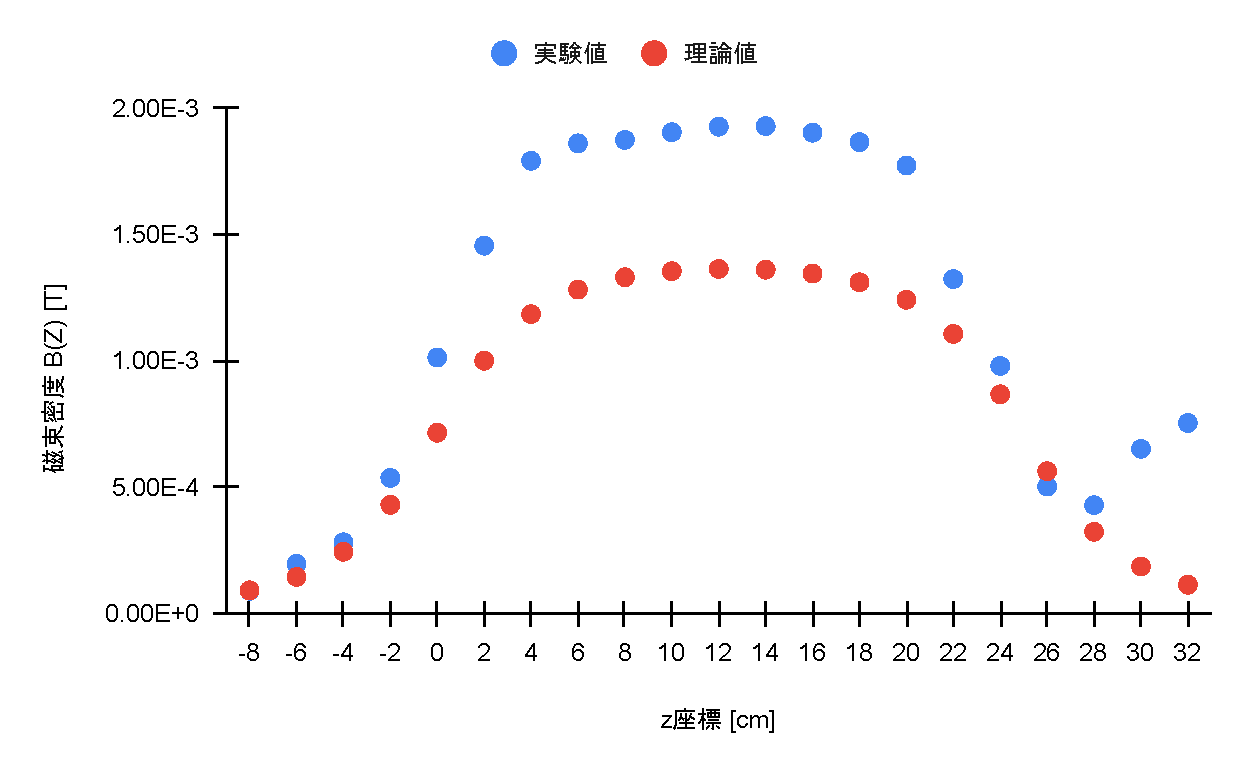
\includegraphics[scale=0.75]{compare.pdf}
            \caption{設問(1)および(2)におけるソレノイド中心軸上の磁束密度分布$B_z(z)$}
        \end{figure}

        \begin{table}[H]
            \centering
            \caption{プローブの測定精度の算出結果}
            \begin{tabular}{c|cc|c}
            \hline
                $z座標\,[\si{cm}]$ & 実験値\,$[\si{mT}]$ & 理論値\,$[\si{mT}]$ & $\frac{\delta B}{B}$ \\ \hline
                -8 & 0.0900 & 0.0917 & -0.018 \\ 
                -6 & 0.196 & 0.145 & 0.36 \\ 
                -4 & 0.282 & 0.244 & 0.15 \\ 
                -2 & 0.537 & 0.430 & 0.25 \\ 
                0 & 1.01 & 0.716 & 0.42 \\ 
                2 & 1.46 & 1.00 & 0.46 \\ 
                4 & 1.79 & 1.18 & 0.51 \\ 
                6 & 1.86 & 1.28 & 0.45 \\ 
                8 & 1.87 & 1.33 & 0.41 \\ 
                10 & 1.91 & 1.36 & 0.41 \\ 
                12 & 1.93 & 1.36 & 0.41 \\ 
                14 & 1.93 & 1.36 & 0.42 \\ 
                16 & 1.90 & 1.35 & 0.41 \\ 
                18 & 1.87 & 1.31 & 0.42 \\ 
                20 & 1.77 & 1.24 & 0.43 \\ 
                22 & 1.32 & 1.11 & 0.20 \\ 
                24 & 0.980 & 0.868 & 0.13 \\ 
                26 & 0.503 & 0.563 & -0.11 \\ 
                28 & 0.429 & 0.323 & 0.33 \\ 
                30 & 0.652 & 0.186 & 2.50 \\ 
                32 & 0.754 & 0.114 & 5.62 \\ \hline
            \end{tabular}
        \end{table}
    \end{description}

    \newpage

    \item 実験課題2において,抵抗$R$の両端の電圧波形$V_R$から閉ループ回路に
    流れるパルス電流の最大値を求めよ.導出過程も示すこと.
    \begin{description}
        \item[] 各鎖交数における電圧波形$V_R$におけるピーク電圧$V_{Rmax}$を
        読み取ることで,閉ループ回路に流れるパルス電流の最大値$IR$は以下の式で
        算出される.
        $$
        I_R=\frac{V_{Rmax}}{R}
        $$
        この算出結果を表6に示す.ただし,$R= 10.6\,[\Omega]$である.
        表6より,パルス電流の最大値の最確値は次のように求められる.
        $$
        I_{RS}\simeq 3.35\,[\si{A}]
        $$
        \begin{table}[H]
            \centering
            \caption{抵抗$R$の両端の電圧波形$V_R$から算出したパルス電流の最大値}
            \begin{tabular}{c|c|c}
            \hline
                鎖交数 & $V_R\,[\si{\volt}]$ & パルス電流の最大値$\,[\si{A}]$ \\ \hline
                1 & 36.0 & 3.40 \\ 
                2 & 35.6 & 3.36 \\ 
                3 & 34.8 & 3.28 \\ 
                4 & 35.6 & 3.36 \\ 
                5 & 35.6 & 3.36 \\ \hline
            \end{tabular}
        \end{table}
    \end{description}
    
    \item 実験課題2において,ロゴスキーコイルの出力$V_e$から閉ループ回路に
    流れるパルス電流の最大値を求めよ.導出過程も示すこと.
    \begin{description}
        \item[] 閉ループ回路に流れるパルス電流は以下の式で算出される.
        $$
        i_e=-\frac{l}{\mu_0 nNS}\int_{0}^{t}V_e(t)dt
        $$
        この算出結果を表7に示す.ただし,各パラメータは次のようになる.
        $$
        \mu_0=1.257\times 10^{-6}\,[\si{H/m}],N=219,S=\pi\times 0.11875^2\simeq 0.04430\,[\si{m^2}],l=2\pi\times 0.11875\simeq 0.7461\,[\si{m}]
        $$
        表7より,パルス電流の最大値の最確値は次のように求められる.
        $$
        I_{es}\simeq 3.04\,[\si{A}]
        $$
        \begin{table}[H]
            \centering
            \caption{ロゴスキーコイルの出力$V_e$から算出したパルス電流の最大値}
            \begin{tabular}{c|c|c}
            \hline
                鎖交数 & $\int_{0}^{t}V_e(t)dt\,[\si{\mu \volt}]$ & パルス電流の最大値$\,[\si{A}]$ \\ \hline
                1 & 0.523 & 3.20 \\ 
                2 & 1.09 & 3.33 \\ 
                3 & 1.53 & 3.13 \\ 
                4 & 1.70 & 2.60 \\ 
                5 & 2.39 & 2.92 \\ \hline
            \end{tabular}
        \end{table}
    \end{description}
    
    \newpage

    \item 実験課題2において,閉ループ回路に流れるパルス電流の最大値を,
    閉ループ回路の回路方程式を解くことによって求めよ.導出過程も示すこと.
    \begin{description}
        \item[] 本実験で用いた閉ループ回路の回路方程式は以下のように表される.
        $$
        L\frac{di}{dt}+Ri+\frac{1}{C}\int idt=V
        $$
        ここで,臨界制動波形であることから、$R^2=\frac{4L}{C}$を満たすので,
        閉ループ回路に流れるパルス電流は以下の式で表される.
        $$
        i=e^{-\frac{R}{2L}t}(C_1+C_2t)
        $$
        ここで,初期条件より$t=0$において,$i=0$,$L\frac{di}{dt}=V$
        であるので,$C_1=0$,$C_2=\frac{V}{L}$となる.
        したがって,閉ループ回路に流れるパルス電流は以下の式で算出される.
        $$
        i=\frac{V}{L}te^{-\frac{R}{2L}t}
        $$
        ここで,パルス電流が最大値を取る時の$t$,充電電圧$V$,ソレノイドコイル
        のインダクタンス$L$,可変抵抗$R$の値は,
        $$
        t=
        $$
        となるので,パルス電流の最大値は次のように求められる.
        $$
        i=\frac{V}{L}te^{-\frac{R}{2L}t}=
        $$
    \end{description}
    
    \item 設問(4)~(6)で求めた値を比較し,その妥当性を検討せよ.
    \begin{description}
        \item[] 設問(6)で得られたパルス電流を理論値として,以下の式で相対誤差率を求める.
        $$
        相対誤差率=\frac{測定値-理論値}{理論値}\times 100
        $$
        抵抗$R$の両端にかかる電圧波形$V_R$より算出したパルス電流の相対誤差率は,
        $$
        1
        $$
        となる.
        また,ロゴスキーコイル両端にかかる電圧波形$V_e$より算出したパルス電流の
        相対誤差率は,
        $$
        1
        $$
        となる.
    \end{description}

    \item 実験課題2において,パルス電流が流れている閉ループとロゴスキーコイル
    の間に存在する相互インダクタンス$M$は,式42で与えられる関係を持つ.
    実際に得られた実験値から,相互インダクタンス$M$を求めよ.導出過程も明記すること.
    \begin{description}
        \item[] 42式より$V_e=M\frac{di}{dt}$が成り立ち,この両辺を$t$
        で積分すると以下の式が成り立つ.
        $$
        \int_{0}^{t}V_e(t)dt=Mi
        $$
    \end{description}

    \item 相互インダクタンス$M$は,式41,42からも分かるように,ロゴスキーコイル
    の形状から求めることが出来る.実際に実測した値から相互インダクタンス$M$を
    算出せよ.導出過程も示すこと.
    \begin{description}
        \item[] $i=\frac{1}{M}\int_{0}^{t}V_e(t)dt$であるので,
        $$
        \frac{l}{\mu_0 NS}\int_{0}^{t}V_e(t)dt=\frac{1}{M}\int_{0}^{t}V_e(t)dt
        $$
        となる.したがって,この式を変形すると相互インダクタンス$M$は以下の式で
        算出される.
        $$
        M=\frac{\mu_0 NS}{l}
        $$
        ただし,各パラメータは次のようになる.
        $$
        \mu_0=1.257\times 10^{-6}\,[\si{H/m}],N=219,S=\pi\times 0.11875^2\simeq 0.04430\,[\si{m^2}],l=2\pi\times 0.11875\simeq 0.7461\,[\si{m}]
        $$
        相互インダクタンス$M$は次のように求められる.
        $$
        M\simeq 1.63\times 10^{-5}\,[\si{H}]
        $$
    \end{description}

    \item 設問(8)および(9)で算出した値を比較し,その妥当性を検討せよ.
    \begin{description}
        \item[] 設問(9)で得られた相互インダクタンスを理論値として,以下の式で相対誤差率を求める.
        $$
        相対誤差率=\frac{測定値-理論値}{理論値}\times 100
        $$
        相互インダクタンス$M$の相対誤差率は,
        $$
        1
        $$
        となる.
    \end{description}

    \item このロゴスキーコイルの形状が円ではなく,楕円のとき,得られる出力はどう
    変化するか答えよ.
    \begin{description}
        \item[] ロゴスキーコイルの原理は,アンペールの周回積分の法則を用いて考えられる.
        そして,アンペールの周回積分の法則は,ループの形状によらないため,ロゴスキーコイルの形状
        が円ではなく,楕円であったとしても,得られる出力は変わらないと考えられる.
    \end{description}
\end{enumerate}